% Use only LaTeX2e, calling the article.cls class and 12-point type.

\documentclass[12pt]{article}

% Users of the {thebibliography} environment or BibTeX should use the
% scicite.sty package, downloadable from *Science* at
% www.sciencemag.org/about/authors/prep/TeX_help/ .
% This package should properly format in-text
% reference calls and reference-list numbers.

\usepackage{scicite}
\usepackage{graphicx}
\usepackage{hyperref}


% Use times if you have the font installed; otherwise, comment out the
% following line.

\usepackage{times}

% The preamble here sets up a lot of new/revised commands and
% environments.  It's annoying, but please do *not* try to strip these
% out into a separate .sty file (which could lead to the loss of some
% information when we convert the file to other formats).  Instead, keep
% them in the preamble of your main LaTeX source file.


% The following parameters seem to provide a reasonable page setup.

\topmargin 0.0cm
\oddsidemargin 0.2cm
\textwidth 16cm 
\textheight 21cm
\footskip 1.0cm


%The next command sets up an environment for the abstract to your paper.

\newenvironment{sciabstract}{%
\begin{quote} \bf}
{\end{quote}}


% If your reference list includes text notes as well as references,
% include the following line; otherwise, comment it out.

\renewcommand\refname{References and Notes}

% The following lines set up an environment for the last note in the
% reference list, which commonly includes acknowledgments of funding,
% help, etc.  It's intended for users of BibTeX or the {thebibliography}
% environment.  Users who are hand-coding their references at the end
% using a list environment such as {enumerate} can simply add another
% item at the end, and it will be numbered automatically.

\newcounter{lastnote}
\newenvironment{scilastnote}{%
\setcounter{lastnote}{\value{enumiv}}%
\addtocounter{lastnote}{+1}%
\begin{list}%
{\arabic{lastnote}.}
{\setlength{\leftmargin}{.22in}}
{\setlength{\labelsep}{.5em}}}
{\end{list}}


% Include your paper's title here

\title{The length of words reflects their conceptual complexity} 


% Place the author information here.  Please hand-code the contact
% information and notecalls; do *not* use \footnote commands.  Let the
% author contact information appear immediately below the author names
% as shown.  We would also prefer that you don't change the type-size
% settings shown here.

\author
{Molly L. Lewis and Michael C. Frank\\
\\
\normalsize{Psychology Department, Stanford University,}\\
\normalsize{450 Serra Mall, Stanford, CA 94305, USA}\\
\\
\normalsize{$^\ast$To whom correspondence should be addressed; E-mail:  mll@stanford.edu.}
}

% Include the date command, but leave its argument blank.

\date{}



%%%%%%%%%%%%%%%%% END OF PREAMBLE %%%%%%%%%%%%%%%%



\begin{document} 

% Double-space the manuscript.

\baselineskip24pt

% Make the title.

\maketitle 



% Place your abstract within the special {sciabstract} environment.

\begin{sciabstract}
Are the forms of words systematically related to their meaning? The arbitrariness of the sign has long been a foundational part of our understanding of human language \cite{saussure,hockett1960}. Theories of communication predict a relationship between length and meaning, however: Longer descriptions should be more conceptually complex\cite{horn1984, levy2006}. Here we show that both the lexicons of human languages and individual speakers encode the relationship between linguistic and conceptual complexity. While word lengths are systematically related to usage---both frequency\cite{zipf1936} and contextual predictability\cite{piantadosi2011a}---our results reveal a systematic relationship with meaning as well. They point to a general regularity in the design of lexicons and reinforce the importance of cognitive constraints on language evolution \cite{christiansen2008,kirby2007,lieberman2007}.
\end{sciabstract}

Human languages are systems for signaling information. A defining feature of these systems is that they are inherently symmetric at all levels. There is no reason to associate a particular form---whether an utterance, a word, or a phoneme---with a particular meaning. Horn\cite{horn1984} observed that pragmatic language users tend to solve this problem of symmetry in a specific way: by considering the effort that speakers have exerted to convey a meaning.  For example, the utterance ``Lee got the car to stop'' seems to imply an unusual state of affairs. Had the speaker wished to convey that Lee simply applied the brakes, the shorter and less exceptional ``Lee stopped the car'' would be a better description. The use of a longer utterance licenses the inference that there was some problem in stopping---perhaps the brakes failed---and that the situation is more complex. Do we reason the same way about the meanings of words, breaking the symmetry between two unknown meanings by reference to length? In other words, is a ``tupabugorn'' more likely to be a complex, unusual object than a ``ralex''? 


\begin{figure}[t!]
\begin{center}
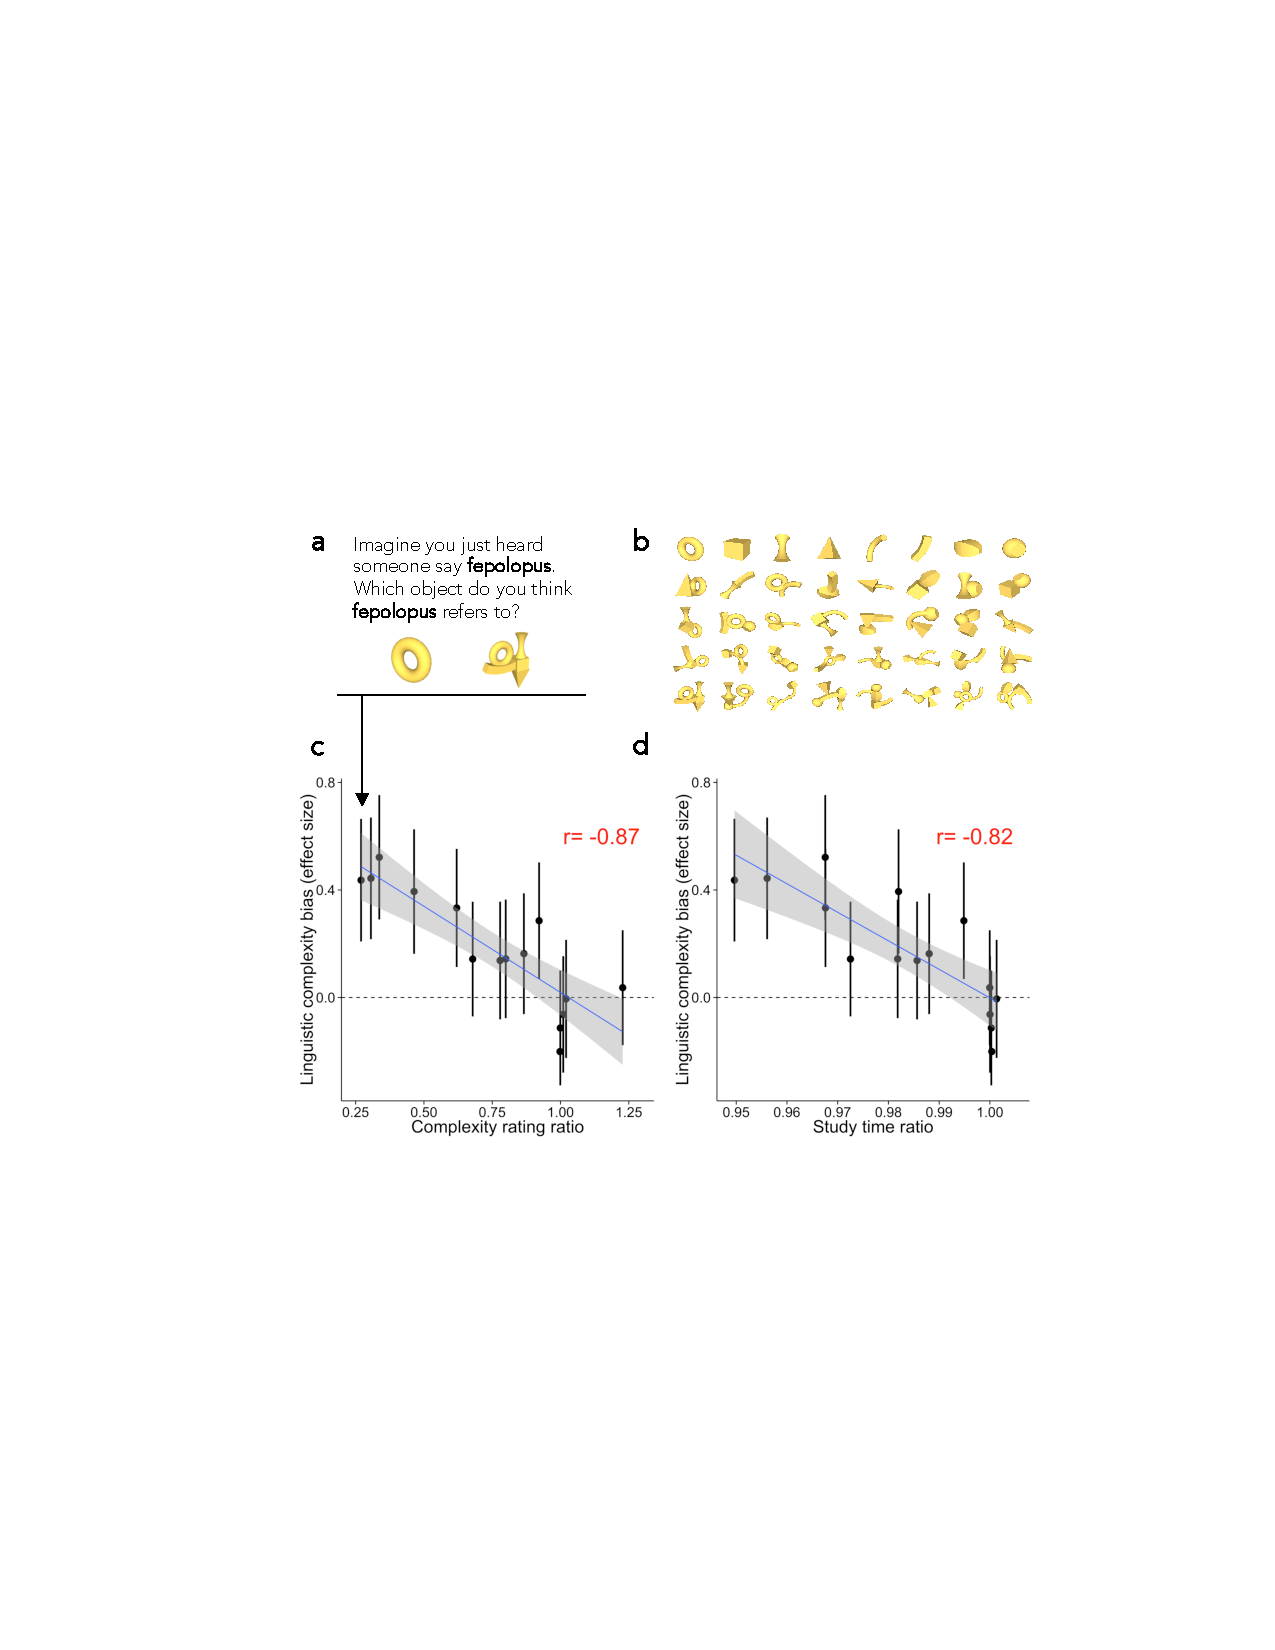
\includegraphics{figs/FIG_1.pdf}
\caption{(a) Schema of a 1 vs.\ 5 geon trial and the corresponding data point. One referential alternative contains one geon and the other contains five geons. (b) Artificial ``geon" stimuli. Each row shows a different level of complexity, determined by the number of geon parts in the objects. (c, d) Experimental results from a task in which participants were asked to map a novel word of varying length to one of two possible referents ($n=750$). Effect size between the long and short language conditions is plotted against the complexity ratio of the two referent alternatives. Fig.\ 1c shows the referents plotted in terms of explicit complexity judgements, and Fig.\ 1d shows the referents plotted in terms of study time. Effect sizes were calculated using the log odds ratio (see Supplementary Materials for further details). Error bars show 95\% confidence intervals.}
\end{center}
\end{figure}

We tested this hypothesis by asking whether speakers would be biased to interpret a long novel word as being more likely to refer to a more complex novel referent. We presented participants on Amazon Mechanical Turk with a novel word of either 2 or 4 syllables and two possible objects as referents (Study 1: $n = 750$; Fig.\ 1a). Possible referents were novel artificial objects whose complexity we manipulated by varying the number of parts the object contained (1 - 5 ``geons'' \cite{biederman1987}; Fig.\ 1b; these judgements were highly correlated with explicit complexity judgments, Study 2: $n = 60$, $r = .93$, $p < .0001$). Participants were asked to select which object the word named for every unique combination of object complexities (1 vs.\ 2 geons, 1 vs.\ 3 geons, 1 vs.\ 4 geons, etc.).

Across conditions, the more complex object was more likely to be judged the referent of the longer word. For each object condition (e.g., 1 vs.\ 2 geons), we calculated the effect size for participants' complexity bias---the degree to which the complex object was more likely to be chosen as the referent of a long word, compared to the short word. Effect size was highly correlated with the ratio of object complexities: The greater the mismatch in object complexity, the more the longer word was paired with the more complex object ($r = -.87$, $p < .0001$; Fig.\ 1c). In a control experiment, we also found this bias with words that were composed of randomly concatenated syllables: participants were more likely to select a five geon object compared to a single geon object as the number of syllables in the word increased (Study 3: $n = 200$; $\beta=-.44$, $p <.0001$).
					

Next we asked whether this bias extended to more naturalistic objects. We gathered a sample of real objects without canonical labels (Fig.\ 2a) and asked participants to rate their complexity. These judgements were highly reliable across two independent samples (Study 4: $n = 60$ in each, $r = .93$, $p < .0001$). We then divided the objects into quintiles based on these ratings, and used them as stimuli in a mapping task identical to the one used with the artificial objects. As with the artificial objects, effect size was negatively correlated with the complexity rating ratio between the referent alternatives (Study 5: $n = 1500$; $r = .70$, $p < .005$; Fig.\ 2b). We also replicated this result with randomly concatenated syllables, such that participants were more likely to select an object from the fifth quintile as opposed to the first quintile when the novel word contained more syllables (Study 6: $n=200$, $\beta=-.34,$ $p <.0001$). Finally, we  found the same bias in language production: Participants produced novel coinages that were longer for the top quartile of objects compared to the bottom quartile (Study 7: $n = 59$; $t(57) = 3.92$, $p < .001$). 

	
If complexity is related to a basic cognitive process, we should be able to measure it using an implicit task, not just via explicit ratings. In visual cognition, stimuli that contain more information require more processing time in search \cite{alvarez2004capacity, hyman}. To test this prediction, we measured participants' study time of objects in a memory task. Each participant studied half of the objects in the stimulus set, one at a time, and then made old/new judgments for the entire set. Critically, the study phase was self-paced, such that participants were allowed to study each object for as much time as they wanted. This study time provided an implicit measure of complexity.

\begin{figure}[t!]
\begin{center}
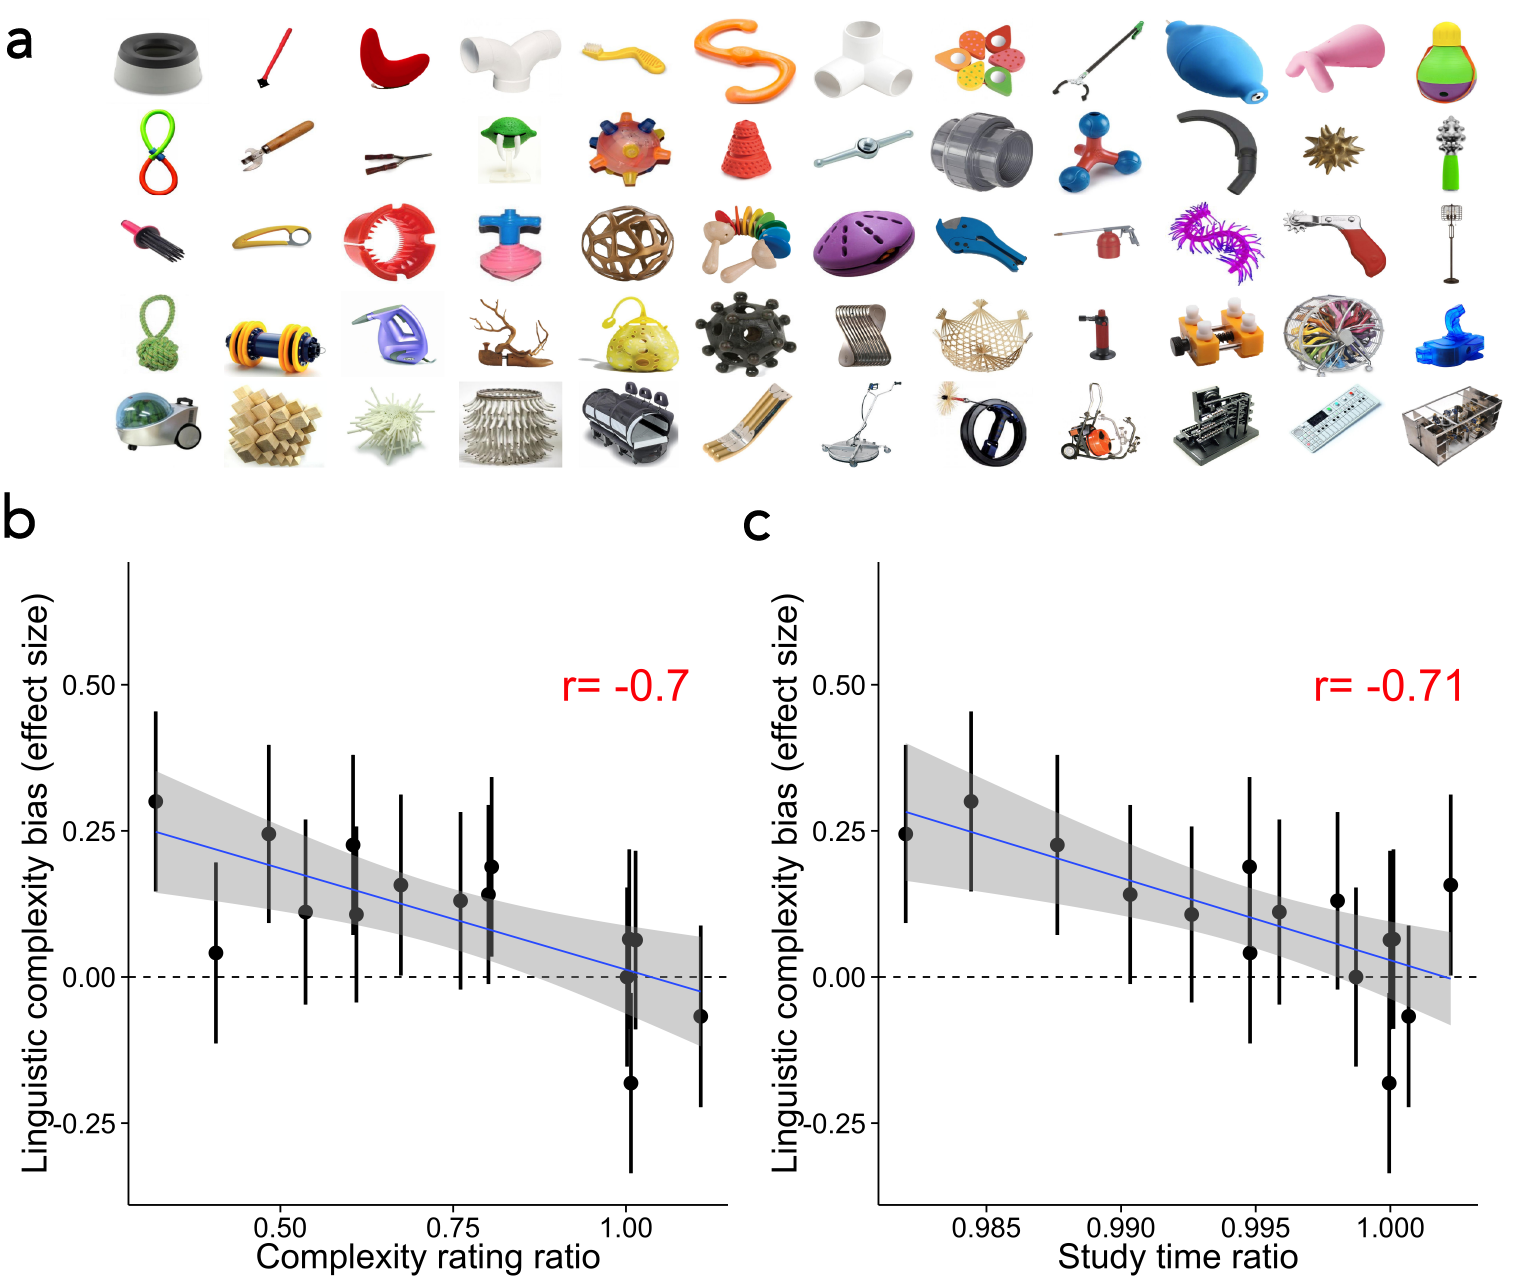
\includegraphics{figs/FIG_2.png}
\caption{(a) Naturalistic, novel stimuli. Each row corresponds to a quintile determined by the explicit complexity judgements (top: least complex; bottom: most complex). (b, c) Experimental results from a task in which participants were asked to map a novel word of varying length to one of two possible referents ($n=1500$). Effect size between the long and short language conditions is plotted against the complexity ratio of the two referent alternatives. Fig.\ 2b shows the referents plotted in terms of explicit complexity judgements, and Fig.\ 2c shows the referents plotted in terms of study time. Effect sizes were calculated using the log odds ratio (see Supplementary Materials for further details). Error bars show 95\% confidence intervals.}
\end{center}
\end{figure}

Mean study time was highly correlated with explicit complexity norms for both artificial objects (Study 8: $n = 250$; $r = .89$, $p < .0001$) and novel real objects (Study 9: $n = 500$; $r = .54$, $p < .0001$). In addition, the ratio of study times for the two object alternatives was correlated with the bias to choose a longer label for both the artificial objects ($r = .82$, $p < .001$; Fig.\ 1c) and the novel real objects ($r = .71$, $p < .005$; Fig.\ 2c): Relatively longer study times predicted longer labels. These findings suggest that label judgments are supported by basic cognitive processes related to the complexity or information content of a stimulus. 
					
Together, these experiments point to a complexity bias in interpreting novel labels: Words that are longer tend to be associated with meanings that are more complex, as reflected in both explicit and implicit measures. Is this bias only relevant to judgments of unfamiliar words, or does it apply to familiar labels as well? 

We collected ratings of meaning complexity for 499 English words in a rating procedure similar to the objects in Studies 2 and 4 (Study 10: $n = 246$). Complexity judgements were positively correlated with word length, measured in phonemes, syllables, and morphemes ($r_{phonemes} = .67$, $r_{syllables} = .63$, $r_{morphemes} = .43$, all $p$s $< .0001$), even when closed-class words were excluded ($n = 438$; $r_{phonemes} = .65$, $r_{syllables} = .63$, $r_{morphemes} = .42$, all $p$s $< .0001$). Importantly, these relationships also remained reliable after controlling for the word's concreteness, imageability, and familiarity. 
						
If the complexity bias relies on a universal cognitive process, it should generalize to lexicons beyond English. We explored this prediction in 79 additional languages, using Google Translate to translate our word set (Study 11). Native speakers checked the accuracy of these translations for 12 of the 79 languages, finding an accuracy of .92 within this sample. For each language, we calculated the correlation between word length in terms of number of characters (to allow comparison between languages for which no phonetic dictionary was available) and mean complexity rating. All 79 languages showed a positive correlation between length and complexity ratings (Fig. 3). The grand mean correlation across languages was .34. 
					

Word length is strongly related to linguistic predictability, operationalized via simple frequency \cite{zipf1936} or using a language model \cite{piantadosi2011a}. But the regularity we describe---a relationship between conceptual complexity and word length---holds even when controlling for frequency. In English, the correlation was only slightly reduced when controlling for log frequency ($r = .57$, $p < .0001$). Across languages, partialling out log frequency (estimated in English), the grand mean correlation was .22. In addition, when we manipulated the observed frequencies of novel objects experimentally, we found no effects on judgments of word length (Studies 12--13). 

\begin{figure}[t!]
\begin{center}
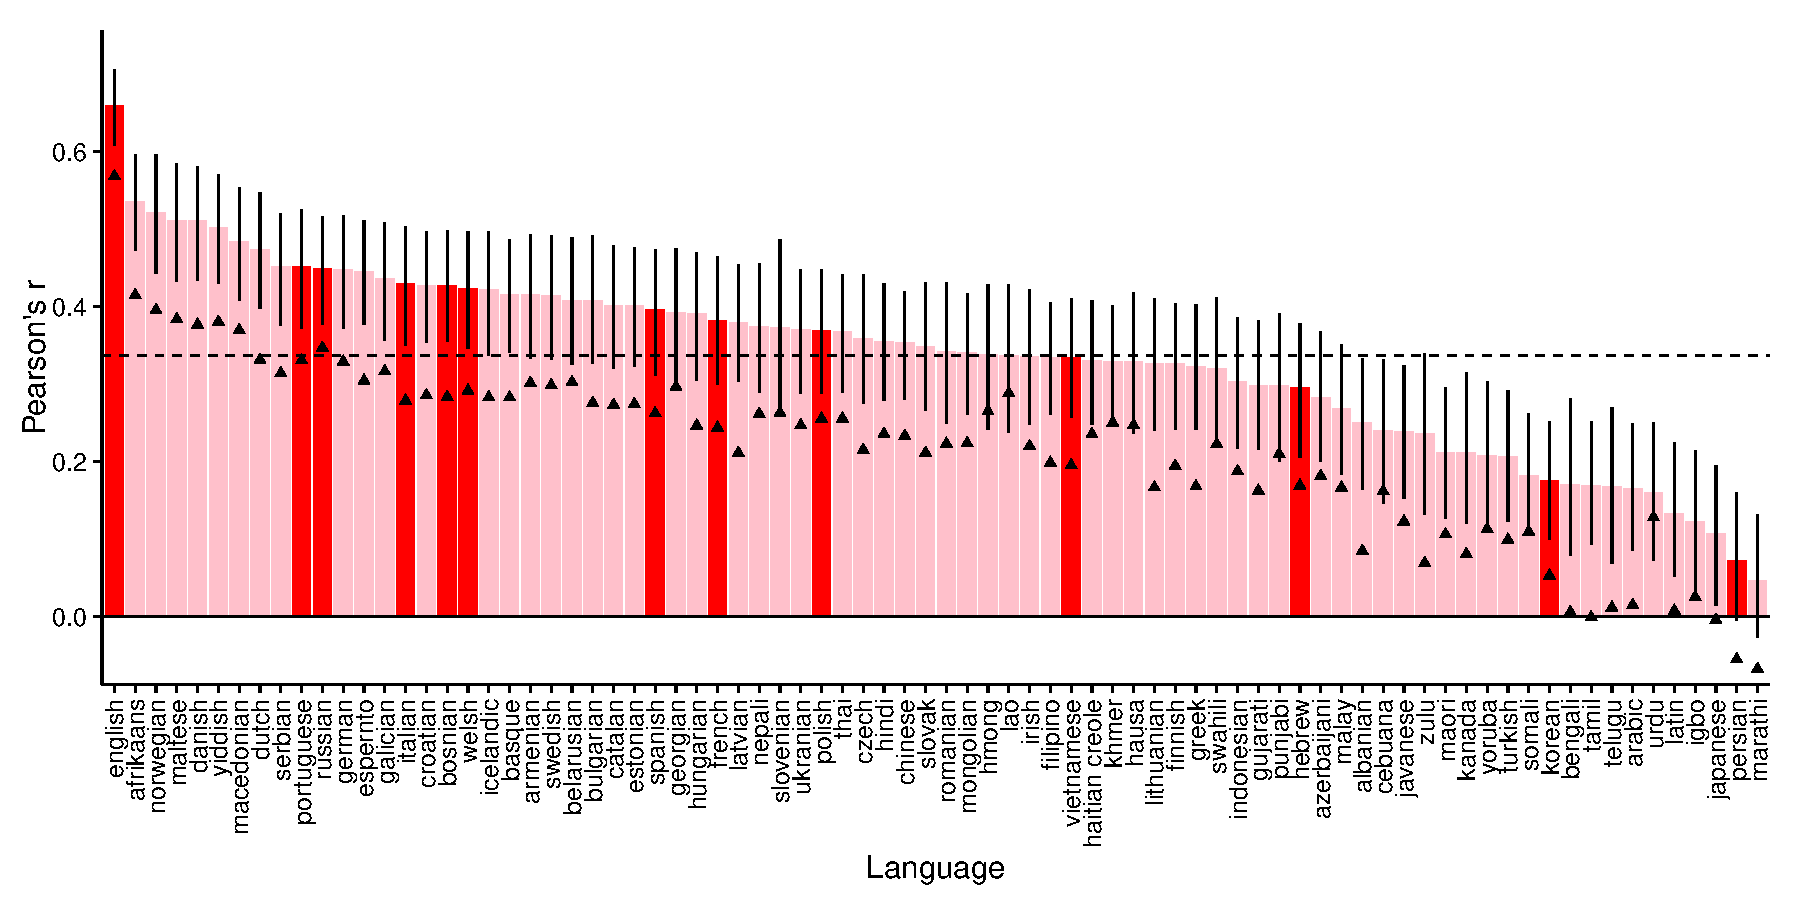
\includegraphics[scale = .53]{figs/FIG_3.pdf}
\caption{Correlations between conceptual complexity norms and word lengths, across languages. Dark red bars indicate languages for which translations were checked by native speakers; all other bars show translations obtained via Google Translate. Error bars show 95\% confidence intervals obtained via non-parametric bootstrap. Triangles indicate correlation value partialling out English log frequency. The dashed line indicates the grand mean correlation across languages.} 
\end{center}
\end{figure}
				

Languages also show phonological iconicity effects, such that semantic features \cite{maurer2006shape} and even particular form classes \cite{farmer2006phonological} are marked by particular sound patterns. However, the type of iconicity explored here is broader---a systematic relationship between abstract measures of complexity and amount of verbal or orthographic effort. Specific iconic hypotheses that posit a parallel between an object's parts and the number of phonemes, morphemes, or syllables in its label do not account for the patterns in the English lexicon: The length-complexity correlation holds even more strongly for words below the median in concreteness, those words whose part structure is presumably much less obvious ($r_{phonemes}= .73$, $r_{syllables} = .72$, $r_{morphemes} = .47$, all $p$s $< .0001$). 

Greenberg\cite{greenberg1966} noted that some forms are more complex, or \emph{marked}, where markedness is denoted by morphological structure. For example, on this account, plurals are considered more complex than singulars because they are more marked morphologically (by the -s morpheme). Although this difference in the complexity of morphological structure could in principle contribute to conceptual complexity judgments, it does not explain the pattern in our data. First, if participants' conceptual complexity judgements were based on English morphological complexity, we should not expect to see correlations between those judgments and word length in other, unrelated languages like Basque or Mandarin. Second, in English, the correlations we observed hold for words with no obvious derivational morphology (CELEX2 monomorphemes \cite{baayen1995celex2}, $n = 387$; $r_{phonemes} = .53$, $r_{syllables} = .47$, all $p$s $< .0001$). 

The regularity that Horn described \cite{horn1984}---that longer sentences are inferred to have more complex or unusual meanings---provides a method for breaking the symmetry inherent in arbitrary signaling systems. Our work here suggests that the lexicons of natural languages break their symmetry via this same regularity: Word length is systematically related to the cognitive complexity of referents. Our data do not speak to the processes underlying participants' judgments---these judgments need not reflect in-the-moment pragmatic inference; they could also be the result of an iconic mapping between effort and meaning, or a lower-level statistical regularity extracted through extensive experience with a language. Regardless of the cognitive instantiation of this inference, the result is lexicons that reflect Horn's principle. 

% Supplemental Materials references
\nocite{crump2013evaluating}
\nocite{sanchez2003effect}
\nocite{wilson1988mrc}
\nocite{brysbaert2009moving}

\bibliography{biblibrary}
\bibliographystyle{Science}

\subsection*{Acknowledgments}
We gratefully acknowledge the support of ONR Grant N00014-13-1-0287. The data reported in this paper are tabulated in the Supplementary Material and archived at the following database: \url{https://github.com/mllewis/RC}.  The authors declare no competing financial interests. MLL and MCF designed research. MLL conducted research. MLL and MCF wrote the paper.

\subsection*{Supplementary Materials}
Supplementary Materials can be found at \url{http://rpubs.com/mll/50311}.\\
Methods and Supplemental Text\\
References (17-20)

\end{document}

